Так как в случае лабораторного источника рентгеновское излучение имеет
некое угловое  (см. \ref{sec:source_section}) и спектральное распределение,
для рентгенодифракционных исследований требуется монохроматор, принцип действия которого
был описан в разделе \ref{sec:single_crystal_section}. Исходный пучок, отражаясь от
кристалла (схема на рис. \ref{ris:single_crystal_schem_lamtet}), разделятся в пространстве
в соответствие с условием Вульфа-Брэгга.
% В рамках последовательно движения от более простого к более сложному мы не оставили без внимание
% получения угловой зависимости интенсивности (рис. \ref{ris:single_crystal_schem_exp}), чтобы соотнести
% выражение для описания спектра трубки (\ref{eq:source_spectral}) с экспериментальным.

\begin{figure}[H]
  \centering
  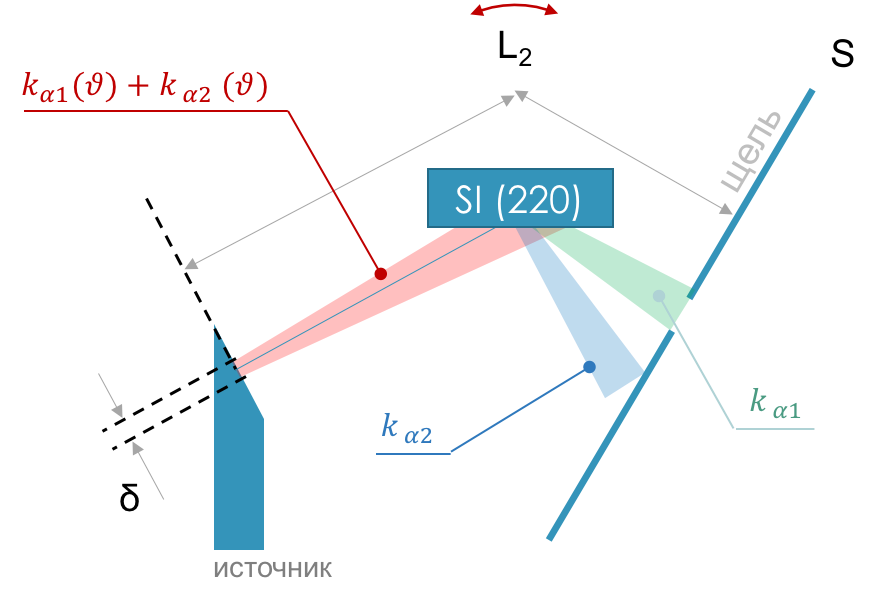
\includegraphics[width=0.5\textwidth]{images/single_crystal_schem_exp.png}
  \caption{ПРинцип действия монокристального монохроматора: лучи с разной энергией отражаются под разными углами
  в соответсвии с законон Вульфа-Брэгга}
  \label{ris:single_crystal_schem_exp}
\end{figure}
%
Угловое распределение характеристического излучения после его отражения от монохроматора (по сути,
вид спектра источника излучения) может быть получено в эксперименте с помощью двух видов сканирования:
поворота образца при неподвижном детекторе, либо сканированием разложенного в пространстве
с помощью монохроматора спектра посредством поворота детектора с установленной перед ним узкой щелью.

На рис. \ref{ris:zero_exp} представлен вид спектра рентгеновской трубки с молибденовым анодом,
полученный путем первого вида сканирования. В качестве монохроматора был использован Si(220)
% Интенсивности отражения рентгеновского излучения приведенная на рис. \ref{ris:zero_exp} может быть
% получена в зависимость от угла поворота кристалла или движение детектор с щелевым устройством,
% задающим его апертуру. В качестве кристалла был взят монокристалл кремния Si(220).

\begin{figure}[H]
  \centering
  \subfloat[]{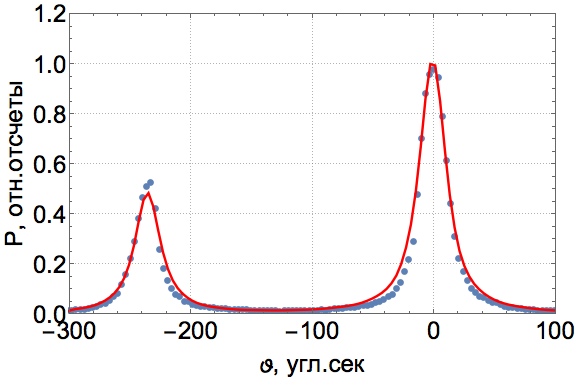
\includegraphics[width=0.45\textwidth]{images/single_cr_exp_s_005mm.png}}
  \hfill
  \subfloat[]{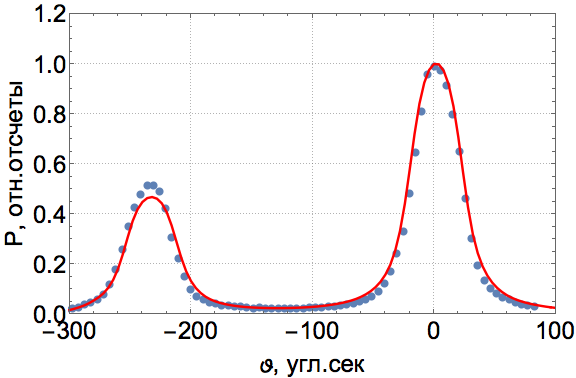
\includegraphics[width=0.45\textwidth]{images/single_cr_exp_s_02mm.png}}
  \caption{Угловая зависимость интенсивности рентгеновского излучения
  после отражения характерестического излучения от кристалла монохроматора:
  расчет -  (красная линия), эксперимент - (синие точки) для $S = 50$ мкм; полуширина $k_{\alpha 1}$ линии ($\vartheta=0$)
   составляет около 30 угл.сек. (a), $S = 200$ мкм; полуширина $k_{\alpha 1}$ линии ($\vartheta=0$)
   составляет около 50 угл.сек. (b)}
  \label{ris:zero_exp}
\end{figure}

Результат сравнения экспериментальной картины дифракции и моделирования
подтверждает правильность выбора функции спектра рентгеновской трубки (\ref{eq:source_spectral}),
в виде суммы двух функций Лоренца, взятых с весовыми коэффициентами. Также из
сравнения экспериментальных и расчетных данных можно сделать вывод, что тормозным
излучением рентгеновской трубки при расчетах можно пренебречь.
